\documentclass[twoside]{book}

% Packages required by doxygen
\usepackage{fixltx2e}
\usepackage{calc}
\usepackage{doxygen}
\usepackage[export]{adjustbox} % also loads graphicx
\usepackage{graphicx}
\usepackage[utf8]{inputenc}
\usepackage{makeidx}
\usepackage{multicol}
\usepackage{multirow}
\PassOptionsToPackage{warn}{textcomp}
\usepackage{textcomp}
\usepackage[nointegrals]{wasysym}
\usepackage[table]{xcolor}

% Font selection
\usepackage[T1]{fontenc}
\usepackage[scaled=.90]{helvet}
\usepackage{courier}
\usepackage{amssymb}
\usepackage{sectsty}
\renewcommand{\familydefault}{\sfdefault}
\allsectionsfont{%
  \fontseries{bc}\selectfont%
  \color{darkgray}%
}
\renewcommand{\DoxyLabelFont}{%
  \fontseries{bc}\selectfont%
  \color{darkgray}%
}
\newcommand{\+}{\discretionary{\mbox{\scriptsize$\hookleftarrow$}}{}{}}

% Page & text layout
\usepackage{geometry}
\geometry{%
  a4paper,%
  top=2.5cm,%
  bottom=2.5cm,%
  left=2.5cm,%
  right=2.5cm%
}
\tolerance=750
\hfuzz=15pt
\hbadness=750
\setlength{\emergencystretch}{15pt}
\setlength{\parindent}{0cm}
\setlength{\parskip}{0.2cm}
\makeatletter
\renewcommand{\paragraph}{%
  \@startsection{paragraph}{4}{0ex}{-1.0ex}{1.0ex}{%
    \normalfont\normalsize\bfseries\SS@parafont%
  }%
}
\renewcommand{\subparagraph}{%
  \@startsection{subparagraph}{5}{0ex}{-1.0ex}{1.0ex}{%
    \normalfont\normalsize\bfseries\SS@subparafont%
  }%
}
\makeatother

% Headers & footers
\usepackage{fancyhdr}
\pagestyle{fancyplain}
\fancyhead[LE]{\fancyplain{}{\bfseries\thepage}}
\fancyhead[CE]{\fancyplain{}{}}
\fancyhead[RE]{\fancyplain{}{\bfseries\leftmark}}
\fancyhead[LO]{\fancyplain{}{\bfseries\rightmark}}
\fancyhead[CO]{\fancyplain{}{}}
\fancyhead[RO]{\fancyplain{}{\bfseries\thepage}}
\fancyfoot[LE]{\fancyplain{}{}}
\fancyfoot[CE]{\fancyplain{}{}}
\fancyfoot[RE]{\fancyplain{}{\bfseries\scriptsize Generated on Mon May 18 2015 18\+:12\+:47 for Py\+Caffe by Doxygen }}
\fancyfoot[LO]{\fancyplain{}{\bfseries\scriptsize Generated on Mon May 18 2015 18\+:12\+:47 for Py\+Caffe by Doxygen }}
\fancyfoot[CO]{\fancyplain{}{}}
\fancyfoot[RO]{\fancyplain{}{}}
\renewcommand{\footrulewidth}{0.4pt}
\renewcommand{\chaptermark}[1]{%
  \markboth{#1}{}%
}
\renewcommand{\sectionmark}[1]{%
  \markright{\thesection\ #1}%
}

% Indices & bibliography
\usepackage{natbib}
\usepackage[titles]{tocloft}
\setcounter{tocdepth}{3}
\setcounter{secnumdepth}{5}
\makeindex

% Hyperlinks (required, but should be loaded last)
\usepackage{ifpdf}
\ifpdf
  \usepackage[pdftex,pagebackref=true]{hyperref}
\else
  \usepackage[ps2pdf,pagebackref=true]{hyperref}
\fi
\hypersetup{%
  colorlinks=true,%
  linkcolor=blue,%
  citecolor=blue,%
  unicode%
}

% Custom commands
\newcommand{\clearemptydoublepage}{%
  \newpage{\pagestyle{empty}\cleardoublepage}%
}


%===== C O N T E N T S =====

\begin{document}

% Titlepage & ToC
\hypersetup{pageanchor=false,
             bookmarks=true,
             bookmarksnumbered=true,
             pdfencoding=unicode
            }
\pagenumbering{roman}
\begin{titlepage}
\vspace*{7cm}
\begin{center}%
{\Large Py\+Caffe }\\
\vspace*{1cm}
{\large Generated by Doxygen 1.8.9}\\
\vspace*{0.5cm}
{\small Mon May 18 2015 18:12:47}\\
\end{center}
\end{titlepage}
\clearemptydoublepage
\tableofcontents
\clearemptydoublepage
\pagenumbering{arabic}
\hypersetup{pageanchor=true}

%--- Begin generated contents ---
\chapter{Namespace Index}
\section{Namespace List}
Here is a list of all documented namespaces with brief descriptions\+:\begin{DoxyCompactList}
\item\contentsline{section}{\hyperlink{namespacecaffe_1_1draw}{caffe.\+draw} }{\pageref{namespacecaffe_1_1draw}}{}
\item\contentsline{section}{\hyperlink{namespacecaffe_1_1pycaffe}{caffe.\+pycaffe} }{\pageref{namespacecaffe_1_1pycaffe}}{}
\end{DoxyCompactList}

\chapter{Hierarchical Index}
\section{Class Hierarchy}
This inheritance list is sorted roughly, but not completely, alphabetically\+:\begin{DoxyCompactList}
\item \contentsline{section}{caffe\+:\+:Ndarray\+Converter\+Generator\+:\+:apply$<$ T $>$}{\pageref{structcaffe_1_1_ndarray_converter_generator_1_1apply}}{}
\item \contentsline{section}{caffe\+:\+:Ndarray\+Converter\+Generator\+:\+:apply$<$ Dtype $\ast$ $>$}{\pageref{structcaffe_1_1_ndarray_converter_generator_1_1apply_3_01_dtype_01_5_01_4}}{}
\item default\+\_\+call\+\_\+policies\begin{DoxyCompactList}
\item \contentsline{section}{caffe\+:\+:Ndarray\+Call\+Policies}{\pageref{structcaffe_1_1_ndarray_call_policies}}{}
\end{DoxyCompactList}
\item \contentsline{section}{caffe\+:\+:Ndarray\+Converter\+Generator}{\pageref{structcaffe_1_1_ndarray_converter_generator}}{}
\item Test\+Case\begin{DoxyCompactList}
\item \contentsline{section}{test\+\_\+net.\+Test\+Net}{\pageref{classtest__net_1_1_test_net}}{}
\item \contentsline{section}{test\+\_\+python\+\_\+layer.\+Test\+Python\+Layer}{\pageref{classtest__python__layer_1_1_test_python_layer}}{}
\item \contentsline{section}{test\+\_\+solver.\+Test\+Solver}{\pageref{classtest__solver_1_1_test_solver}}{}
\end{DoxyCompactList}
\item \contentsline{section}{caffe.\+io.\+Transformer}{\pageref{classcaffe_1_1io_1_1_transformer}}{}
\item \contentsline{section}{caffe\+:\+:Ndarray\+Converter\+Generator\+:\+:apply$<$ Dtype $\ast$ $>$\+:\+:type}{\pageref{structcaffe_1_1_ndarray_converter_generator_1_1apply_3_01_dtype_01_5_01_4_1_1type}}{}
\item Layer\begin{DoxyCompactList}
\item \contentsline{section}{test\+\_\+python\+\_\+layer.\+Simple\+Layer}{\pageref{classtest__python__layer_1_1_simple_layer}}{}
\end{DoxyCompactList}
\item Net\begin{DoxyCompactList}
\item \contentsline{section}{caffe.\+classifier.\+Classifier}{\pageref{classcaffe_1_1classifier_1_1_classifier}}{}
\item \contentsline{section}{caffe.\+detector.\+Detector}{\pageref{classcaffe_1_1detector_1_1_detector}}{}
\end{DoxyCompactList}
\end{DoxyCompactList}

\chapter{Class Index}
\section{Class List}
Here are the classes, structs, unions and interfaces with brief descriptions\+:\begin{DoxyCompactList}
\item\contentsline{section}{\hyperlink{structcaffe_1_1_ndarray_converter_generator_1_1apply}{caffe\+::\+Ndarray\+Converter\+Generator\+::apply$<$ T $>$} }{\pageref{structcaffe_1_1_ndarray_converter_generator_1_1apply}}{}
\item\contentsline{section}{\hyperlink{structcaffe_1_1_ndarray_converter_generator_1_1apply_3_01_dtype_01_5_01_4}{caffe\+::\+Ndarray\+Converter\+Generator\+::apply$<$ Dtype $\ast$ $>$} }{\pageref{structcaffe_1_1_ndarray_converter_generator_1_1apply_3_01_dtype_01_5_01_4}}{}
\item\contentsline{section}{\hyperlink{classcaffe_1_1classifier_1_1_classifier}{caffe.\+classifier.\+Classifier} }{\pageref{classcaffe_1_1classifier_1_1_classifier}}{}
\item\contentsline{section}{\hyperlink{classcaffe_1_1detector_1_1_detector}{caffe.\+detector.\+Detector} }{\pageref{classcaffe_1_1detector_1_1_detector}}{}
\item\contentsline{section}{\hyperlink{structcaffe_1_1_ndarray_call_policies}{caffe\+::\+Ndarray\+Call\+Policies} }{\pageref{structcaffe_1_1_ndarray_call_policies}}{}
\item\contentsline{section}{\hyperlink{structcaffe_1_1_ndarray_converter_generator}{caffe\+::\+Ndarray\+Converter\+Generator} }{\pageref{structcaffe_1_1_ndarray_converter_generator}}{}
\item\contentsline{section}{\hyperlink{classtest__python__layer_1_1_simple_layer}{test\+\_\+python\+\_\+layer.\+Simple\+Layer} }{\pageref{classtest__python__layer_1_1_simple_layer}}{}
\item\contentsline{section}{\hyperlink{classtest__net_1_1_test_net}{test\+\_\+net.\+Test\+Net} }{\pageref{classtest__net_1_1_test_net}}{}
\item\contentsline{section}{\hyperlink{classtest__python__layer_1_1_test_python_layer}{test\+\_\+python\+\_\+layer.\+Test\+Python\+Layer} }{\pageref{classtest__python__layer_1_1_test_python_layer}}{}
\item\contentsline{section}{\hyperlink{classtest__solver_1_1_test_solver}{test\+\_\+solver.\+Test\+Solver} }{\pageref{classtest__solver_1_1_test_solver}}{}
\item\contentsline{section}{\hyperlink{classcaffe_1_1io_1_1_transformer}{caffe.\+io.\+Transformer} \\*Pre-\/processing }{\pageref{classcaffe_1_1io_1_1_transformer}}{}
\item\contentsline{section}{\hyperlink{structcaffe_1_1_ndarray_converter_generator_1_1apply_3_01_dtype_01_5_01_4_1_1type}{caffe\+::\+Ndarray\+Converter\+Generator\+::apply$<$ Dtype $\ast$ $>$\+::type} }{\pageref{structcaffe_1_1_ndarray_converter_generator_1_1apply_3_01_dtype_01_5_01_4_1_1type}}{}
\end{DoxyCompactList}

\chapter{Namespace Documentation}
\hypertarget{namespacecaffe_1_1draw}{}\section{caffe.\+draw Namespace Reference}
\label{namespacecaffe_1_1draw}\index{caffe.\+draw@{caffe.\+draw}}
\subsection*{Functions}
\begin{DoxyCompactItemize}
\item 
def \hyperlink{namespacecaffe_1_1draw_a3e29c1cd2c9fb6c1cee315b84f9e90e7}{get\+\_\+pooling\+\_\+types\+\_\+dict} ()
\item 
def \hyperlink{namespacecaffe_1_1draw_a7e2ae7989557055211c44b1e9c187daa}{determine\+\_\+edge\+\_\+label\+\_\+by\+\_\+layertype} (layer, layertype)
\item 
def \hyperlink{namespacecaffe_1_1draw_abc4545db9dda6f8d6db7ae56a049de3c}{determine\+\_\+node\+\_\+label\+\_\+by\+\_\+layertype} (layer, layertype, rankdir)
\item 
def \hyperlink{namespacecaffe_1_1draw_a329b4be3aae2dd51158278ea32022512}{choose\+\_\+color\+\_\+by\+\_\+layertype} (layertype)
\item 
\hypertarget{namespacecaffe_1_1draw_a223ae748ac0fe5704e90c938e995572a}{}def {\bfseries get\+\_\+pydot\+\_\+graph}\label{namespacecaffe_1_1draw_a223ae748ac0fe5704e90c938e995572a}

\item 
def \hyperlink{namespacecaffe_1_1draw_af4843d9a765dafcb10193c6165671cb3}{draw\+\_\+net}
\item 
def \hyperlink{namespacecaffe_1_1draw_a28ab49b2cc53904012f304298400df40}{draw\+\_\+net\+\_\+to\+\_\+file}
\end{DoxyCompactItemize}
\subsection*{Variables}
\begin{DoxyCompactItemize}
\item 
dictionary {\bfseries L\+A\+Y\+E\+R\+\_\+\+S\+T\+Y\+L\+E\+\_\+\+D\+E\+F\+A\+U\+L\+T}
\item 
dictionary {\bfseries N\+E\+U\+R\+O\+N\+\_\+\+L\+A\+Y\+E\+R\+\_\+\+S\+T\+Y\+L\+E}
\item 
dictionary {\bfseries B\+L\+O\+B\+\_\+\+S\+T\+Y\+L\+E}
\end{DoxyCompactItemize}


\subsection{Detailed Description}
\begin{DoxyVerb}Caffe network visualization: draw the NetParameter protobuffer.

NOTE: this requires pydot>=1.0.2, which is not included in requirements.txt
since it requires graphviz and other prerequisites outside the scope of the
Caffe.
\end{DoxyVerb}
 

\subsection{Function Documentation}
\hypertarget{namespacecaffe_1_1draw_a329b4be3aae2dd51158278ea32022512}{}\index{caffe\+::draw@{caffe\+::draw}!choose\+\_\+color\+\_\+by\+\_\+layertype@{choose\+\_\+color\+\_\+by\+\_\+layertype}}
\index{choose\+\_\+color\+\_\+by\+\_\+layertype@{choose\+\_\+color\+\_\+by\+\_\+layertype}!caffe\+::draw@{caffe\+::draw}}
\subsubsection[{choose\+\_\+color\+\_\+by\+\_\+layertype}]{\setlength{\rightskip}{0pt plus 5cm}def caffe.\+draw.\+choose\+\_\+color\+\_\+by\+\_\+layertype (
\begin{DoxyParamCaption}
\item[{}]{layertype}
\end{DoxyParamCaption}
)}\label{namespacecaffe_1_1draw_a329b4be3aae2dd51158278ea32022512}
\begin{DoxyVerb}Define colors for nodes based on the layer type
\end{DoxyVerb}
 \hypertarget{namespacecaffe_1_1draw_a7e2ae7989557055211c44b1e9c187daa}{}\index{caffe\+::draw@{caffe\+::draw}!determine\+\_\+edge\+\_\+label\+\_\+by\+\_\+layertype@{determine\+\_\+edge\+\_\+label\+\_\+by\+\_\+layertype}}
\index{determine\+\_\+edge\+\_\+label\+\_\+by\+\_\+layertype@{determine\+\_\+edge\+\_\+label\+\_\+by\+\_\+layertype}!caffe\+::draw@{caffe\+::draw}}
\subsubsection[{determine\+\_\+edge\+\_\+label\+\_\+by\+\_\+layertype}]{\setlength{\rightskip}{0pt plus 5cm}def caffe.\+draw.\+determine\+\_\+edge\+\_\+label\+\_\+by\+\_\+layertype (
\begin{DoxyParamCaption}
\item[{}]{layer, }
\item[{}]{layertype}
\end{DoxyParamCaption}
)}\label{namespacecaffe_1_1draw_a7e2ae7989557055211c44b1e9c187daa}
\begin{DoxyVerb}Define edge label based on layer type
\end{DoxyVerb}
 \hypertarget{namespacecaffe_1_1draw_abc4545db9dda6f8d6db7ae56a049de3c}{}\index{caffe\+::draw@{caffe\+::draw}!determine\+\_\+node\+\_\+label\+\_\+by\+\_\+layertype@{determine\+\_\+node\+\_\+label\+\_\+by\+\_\+layertype}}
\index{determine\+\_\+node\+\_\+label\+\_\+by\+\_\+layertype@{determine\+\_\+node\+\_\+label\+\_\+by\+\_\+layertype}!caffe\+::draw@{caffe\+::draw}}
\subsubsection[{determine\+\_\+node\+\_\+label\+\_\+by\+\_\+layertype}]{\setlength{\rightskip}{0pt plus 5cm}def caffe.\+draw.\+determine\+\_\+node\+\_\+label\+\_\+by\+\_\+layertype (
\begin{DoxyParamCaption}
\item[{}]{layer, }
\item[{}]{layertype, }
\item[{}]{rankdir}
\end{DoxyParamCaption}
)}\label{namespacecaffe_1_1draw_abc4545db9dda6f8d6db7ae56a049de3c}
\begin{DoxyVerb}Define node label based on layer type
\end{DoxyVerb}
 \hypertarget{namespacecaffe_1_1draw_af4843d9a765dafcb10193c6165671cb3}{}\index{caffe\+::draw@{caffe\+::draw}!draw\+\_\+net@{draw\+\_\+net}}
\index{draw\+\_\+net@{draw\+\_\+net}!caffe\+::draw@{caffe\+::draw}}
\subsubsection[{draw\+\_\+net}]{\setlength{\rightskip}{0pt plus 5cm}def caffe.\+draw.\+draw\+\_\+net (
\begin{DoxyParamCaption}
\item[{}]{caffe\+\_\+net, }
\item[{}]{rankdir, }
\item[{}]{ext = {\ttfamily \textquotesingle{}png\textquotesingle{}}}
\end{DoxyParamCaption}
)}\label{namespacecaffe_1_1draw_af4843d9a765dafcb10193c6165671cb3}
\begin{DoxyVerb}Draws a caffe net and returns the image string encoded using the given
extension.

Parameters
----------
caffe_net: a caffe.proto.caffe_pb2.NetParameter protocol buffer.
ext: the image extension. Default 'png'.
\end{DoxyVerb}
 \hypertarget{namespacecaffe_1_1draw_a28ab49b2cc53904012f304298400df40}{}\index{caffe\+::draw@{caffe\+::draw}!draw\+\_\+net\+\_\+to\+\_\+file@{draw\+\_\+net\+\_\+to\+\_\+file}}
\index{draw\+\_\+net\+\_\+to\+\_\+file@{draw\+\_\+net\+\_\+to\+\_\+file}!caffe\+::draw@{caffe\+::draw}}
\subsubsection[{draw\+\_\+net\+\_\+to\+\_\+file}]{\setlength{\rightskip}{0pt plus 5cm}def caffe.\+draw.\+draw\+\_\+net\+\_\+to\+\_\+file (
\begin{DoxyParamCaption}
\item[{}]{caffe\+\_\+net, }
\item[{}]{filename, }
\item[{}]{rankdir = {\ttfamily \textquotesingle{}LR\textquotesingle{}}}
\end{DoxyParamCaption}
)}\label{namespacecaffe_1_1draw_a28ab49b2cc53904012f304298400df40}
\begin{DoxyVerb}Draws a caffe net, and saves it to file using the format given as the
file extension. Use '.raw' to output raw text that you can manually feed
to graphviz to draw graphs.
\end{DoxyVerb}
 \hypertarget{namespacecaffe_1_1draw_a3e29c1cd2c9fb6c1cee315b84f9e90e7}{}\index{caffe\+::draw@{caffe\+::draw}!get\+\_\+pooling\+\_\+types\+\_\+dict@{get\+\_\+pooling\+\_\+types\+\_\+dict}}
\index{get\+\_\+pooling\+\_\+types\+\_\+dict@{get\+\_\+pooling\+\_\+types\+\_\+dict}!caffe\+::draw@{caffe\+::draw}}
\subsubsection[{get\+\_\+pooling\+\_\+types\+\_\+dict}]{\setlength{\rightskip}{0pt plus 5cm}def caffe.\+draw.\+get\+\_\+pooling\+\_\+types\+\_\+dict (
\begin{DoxyParamCaption}
{}
\end{DoxyParamCaption}
)}\label{namespacecaffe_1_1draw_a3e29c1cd2c9fb6c1cee315b84f9e90e7}
\begin{DoxyVerb}Get dictionary mapping pooling type number to type name
\end{DoxyVerb}
 

\subsection{Variable Documentation}
\hypertarget{namespacecaffe_1_1draw_a90ed854dd2a19d06b9843248c390d6a5}{}\index{caffe\+::draw@{caffe\+::draw}!B\+L\+O\+B\+\_\+\+S\+T\+Y\+L\+E@{B\+L\+O\+B\+\_\+\+S\+T\+Y\+L\+E}}
\index{B\+L\+O\+B\+\_\+\+S\+T\+Y\+L\+E@{B\+L\+O\+B\+\_\+\+S\+T\+Y\+L\+E}!caffe\+::draw@{caffe\+::draw}}
\subsubsection[{B\+L\+O\+B\+\_\+\+S\+T\+Y\+L\+E}]{\setlength{\rightskip}{0pt plus 5cm}dictionary caffe.\+draw.\+B\+L\+O\+B\+\_\+\+S\+T\+Y\+L\+E}\label{namespacecaffe_1_1draw_a90ed854dd2a19d06b9843248c390d6a5}
{\bfseries Initial value\+:}
\begin{DoxyCode}
1 = \{\textcolor{stringliteral}{'shape'}: \textcolor{stringliteral}{'octagon'},
2               \textcolor{stringliteral}{'fillcolor'}: \textcolor{stringliteral}{'#E0E0E0'},
3               \textcolor{stringliteral}{'style'}: \textcolor{stringliteral}{'filled'}\}
\end{DoxyCode}
\hypertarget{namespacecaffe_1_1draw_a2d924dfcc48367553fc1a36a9bbfa805}{}\index{caffe\+::draw@{caffe\+::draw}!L\+A\+Y\+E\+R\+\_\+\+S\+T\+Y\+L\+E\+\_\+\+D\+E\+F\+A\+U\+L\+T@{L\+A\+Y\+E\+R\+\_\+\+S\+T\+Y\+L\+E\+\_\+\+D\+E\+F\+A\+U\+L\+T}}
\index{L\+A\+Y\+E\+R\+\_\+\+S\+T\+Y\+L\+E\+\_\+\+D\+E\+F\+A\+U\+L\+T@{L\+A\+Y\+E\+R\+\_\+\+S\+T\+Y\+L\+E\+\_\+\+D\+E\+F\+A\+U\+L\+T}!caffe\+::draw@{caffe\+::draw}}
\subsubsection[{L\+A\+Y\+E\+R\+\_\+\+S\+T\+Y\+L\+E\+\_\+\+D\+E\+F\+A\+U\+L\+T}]{\setlength{\rightskip}{0pt plus 5cm}dictionary caffe.\+draw.\+L\+A\+Y\+E\+R\+\_\+\+S\+T\+Y\+L\+E\+\_\+\+D\+E\+F\+A\+U\+L\+T}\label{namespacecaffe_1_1draw_a2d924dfcc48367553fc1a36a9bbfa805}
{\bfseries Initial value\+:}
\begin{DoxyCode}
1 = \{\textcolor{stringliteral}{'shape'}: \textcolor{stringliteral}{'record'},
2                        \textcolor{stringliteral}{'fillcolor'}: \textcolor{stringliteral}{'#6495ED'},
3                        \textcolor{stringliteral}{'style'}: \textcolor{stringliteral}{'filled'}\}
\end{DoxyCode}
\hypertarget{namespacecaffe_1_1draw_a72f7eccee11a4375210203cf02bea0f8}{}\index{caffe\+::draw@{caffe\+::draw}!N\+E\+U\+R\+O\+N\+\_\+\+L\+A\+Y\+E\+R\+\_\+\+S\+T\+Y\+L\+E@{N\+E\+U\+R\+O\+N\+\_\+\+L\+A\+Y\+E\+R\+\_\+\+S\+T\+Y\+L\+E}}
\index{N\+E\+U\+R\+O\+N\+\_\+\+L\+A\+Y\+E\+R\+\_\+\+S\+T\+Y\+L\+E@{N\+E\+U\+R\+O\+N\+\_\+\+L\+A\+Y\+E\+R\+\_\+\+S\+T\+Y\+L\+E}!caffe\+::draw@{caffe\+::draw}}
\subsubsection[{N\+E\+U\+R\+O\+N\+\_\+\+L\+A\+Y\+E\+R\+\_\+\+S\+T\+Y\+L\+E}]{\setlength{\rightskip}{0pt plus 5cm}dictionary caffe.\+draw.\+N\+E\+U\+R\+O\+N\+\_\+\+L\+A\+Y\+E\+R\+\_\+\+S\+T\+Y\+L\+E}\label{namespacecaffe_1_1draw_a72f7eccee11a4375210203cf02bea0f8}
{\bfseries Initial value\+:}
\begin{DoxyCode}
1 = \{\textcolor{stringliteral}{'shape'}: \textcolor{stringliteral}{'record'},
2                       \textcolor{stringliteral}{'fillcolor'}: \textcolor{stringliteral}{'#90EE90'},
3                       \textcolor{stringliteral}{'style'}: \textcolor{stringliteral}{'filled'}\}
\end{DoxyCode}

\hypertarget{namespacecaffe_1_1pycaffe}{}\section{caffe.\+pycaffe Namespace Reference}
\label{namespacecaffe_1_1pycaffe}\index{caffe.\+pycaffe@{caffe.\+pycaffe}}


\subsection{Detailed Description}
\begin{DoxyVerb}Wrap the internal caffe C++ module (_caffe.so) with a clean, Pythonic
interface.
\end{DoxyVerb}
 
\chapter{Class Documentation}
\hypertarget{structcaffe_1_1_ndarray_converter_generator_1_1apply}{}\section{caffe\+:\+:Ndarray\+Converter\+Generator\+:\+:apply$<$ T $>$ Struct Template Reference}
\label{structcaffe_1_1_ndarray_converter_generator_1_1apply}\index{caffe\+::\+Ndarray\+Converter\+Generator\+::apply$<$ T $>$@{caffe\+::\+Ndarray\+Converter\+Generator\+::apply$<$ T $>$}}


The documentation for this struct was generated from the following file\+:\begin{DoxyCompactItemize}
\item 
caffe/\+\_\+caffe.\+cpp\end{DoxyCompactItemize}

\hypertarget{structcaffe_1_1_ndarray_converter_generator_1_1apply_3_01_dtype_01_5_01_4}{}\section{caffe\+:\+:Ndarray\+Converter\+Generator\+:\+:apply$<$ Dtype $\ast$ $>$ Struct Template Reference}
\label{structcaffe_1_1_ndarray_converter_generator_1_1apply_3_01_dtype_01_5_01_4}\index{caffe\+::\+Ndarray\+Converter\+Generator\+::apply$<$ Dtype $\ast$ $>$@{caffe\+::\+Ndarray\+Converter\+Generator\+::apply$<$ Dtype $\ast$ $>$}}
\subsection*{Classes}
\begin{DoxyCompactItemize}
\item 
struct \hyperlink{structcaffe_1_1_ndarray_converter_generator_1_1apply_3_01_dtype_01_5_01_4_1_1type}{type}
\end{DoxyCompactItemize}


The documentation for this struct was generated from the following file\+:\begin{DoxyCompactItemize}
\item 
caffe/\+\_\+caffe.\+cpp\end{DoxyCompactItemize}

\hypertarget{classcaffe_1_1classifier_1_1_classifier}{}\section{caffe.\+classifier.\+Classifier Class Reference}
\label{classcaffe_1_1classifier_1_1_classifier}\index{caffe.\+classifier.\+Classifier@{caffe.\+classifier.\+Classifier}}
Inheritance diagram for caffe.\+classifier.\+Classifier\+:\begin{figure}[H]
\begin{center}
\leavevmode
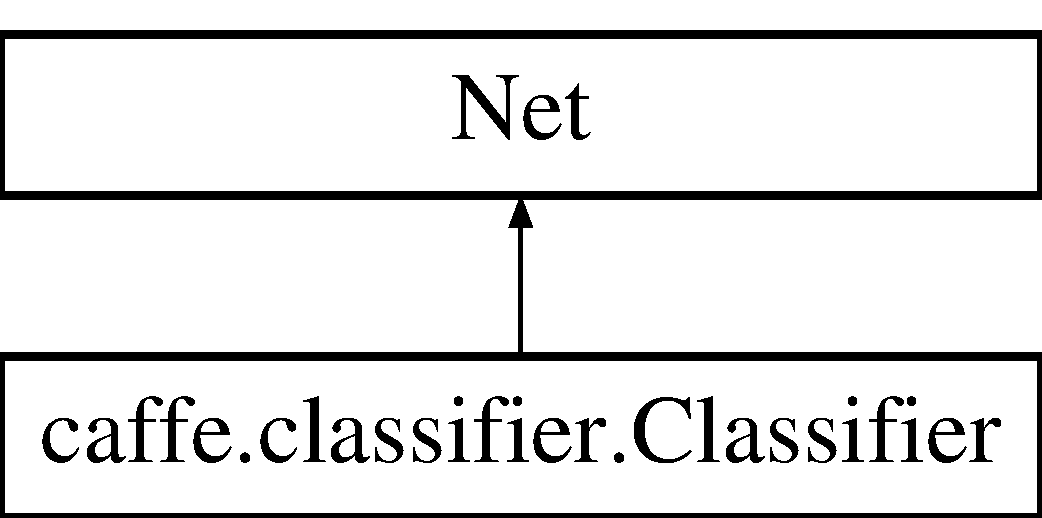
\includegraphics[height=2.000000cm]{classcaffe_1_1classifier_1_1_classifier}
\end{center}
\end{figure}
\subsection*{Public Member Functions}
\begin{DoxyCompactItemize}
\item 
\hypertarget{classcaffe_1_1classifier_1_1_classifier_a2eb5b645a1badd2395b332603d6feb33}{}def {\bfseries \+\_\+\+\_\+init\+\_\+\+\_\+}\label{classcaffe_1_1classifier_1_1_classifier_a2eb5b645a1badd2395b332603d6feb33}

\item 
def \hyperlink{classcaffe_1_1classifier_1_1_classifier_ad888ddf4fb41062925d9e9b919812ce5}{predict}
\end{DoxyCompactItemize}
\subsection*{Public Attributes}
\begin{DoxyCompactItemize}
\item 
\hypertarget{classcaffe_1_1classifier_1_1_classifier_a44a169043638bbf48513fd17dce4f4b6}{}{\bfseries transformer}\label{classcaffe_1_1classifier_1_1_classifier_a44a169043638bbf48513fd17dce4f4b6}

\item 
\hypertarget{classcaffe_1_1classifier_1_1_classifier_a298c47f5b8863db1b3fc06ee3ed0b7ac}{}{\bfseries crop\+\_\+dims}\label{classcaffe_1_1classifier_1_1_classifier_a298c47f5b8863db1b3fc06ee3ed0b7ac}

\item 
\hypertarget{classcaffe_1_1classifier_1_1_classifier_a5e4d8e8e29e3ad083875dfca03c48ba7}{}{\bfseries image\+\_\+dims}\label{classcaffe_1_1classifier_1_1_classifier_a5e4d8e8e29e3ad083875dfca03c48ba7}

\end{DoxyCompactItemize}


\subsection{Detailed Description}
\begin{DoxyVerb}Classifier extends Net for image class prediction
by scaling, center cropping, or oversampling.

Parameters
----------
image_dims : dimensions to scale input for cropping/sampling.
    Default is to scale to net input size for whole-image crop.
mean, input_scale, raw_scale, channel_swap: params for
    preprocessing options.
\end{DoxyVerb}
 

\subsection{Member Function Documentation}
\hypertarget{classcaffe_1_1classifier_1_1_classifier_ad888ddf4fb41062925d9e9b919812ce5}{}\index{caffe\+::classifier\+::\+Classifier@{caffe\+::classifier\+::\+Classifier}!predict@{predict}}
\index{predict@{predict}!caffe\+::classifier\+::\+Classifier@{caffe\+::classifier\+::\+Classifier}}
\subsubsection[{predict}]{\setlength{\rightskip}{0pt plus 5cm}def caffe.\+classifier.\+Classifier.\+predict (
\begin{DoxyParamCaption}
\item[{}]{self, }
\item[{}]{inputs, }
\item[{}]{oversample = {\ttfamily True}}
\end{DoxyParamCaption}
)}\label{classcaffe_1_1classifier_1_1_classifier_ad888ddf4fb41062925d9e9b919812ce5}
\begin{DoxyVerb}Predict classification probabilities of inputs.

Parameters
----------
inputs : iterable of (H x W x K) input ndarrays.
oversample : boolean
    average predictions across center, corners, and mirrors
    when True (default). Center-only prediction when False.

Returns
-------
predictions: (N x C) ndarray of class probabilities for N images and C
    classes.
\end{DoxyVerb}
 

The documentation for this class was generated from the following file\+:\begin{DoxyCompactItemize}
\item 
caffe/classifier.\+py\end{DoxyCompactItemize}

\hypertarget{classcaffe_1_1detector_1_1_detector}{}\section{caffe.\+detector.\+Detector Class Reference}
\label{classcaffe_1_1detector_1_1_detector}\index{caffe.\+detector.\+Detector@{caffe.\+detector.\+Detector}}
Inheritance diagram for caffe.\+detector.\+Detector\+:\begin{figure}[H]
\begin{center}
\leavevmode
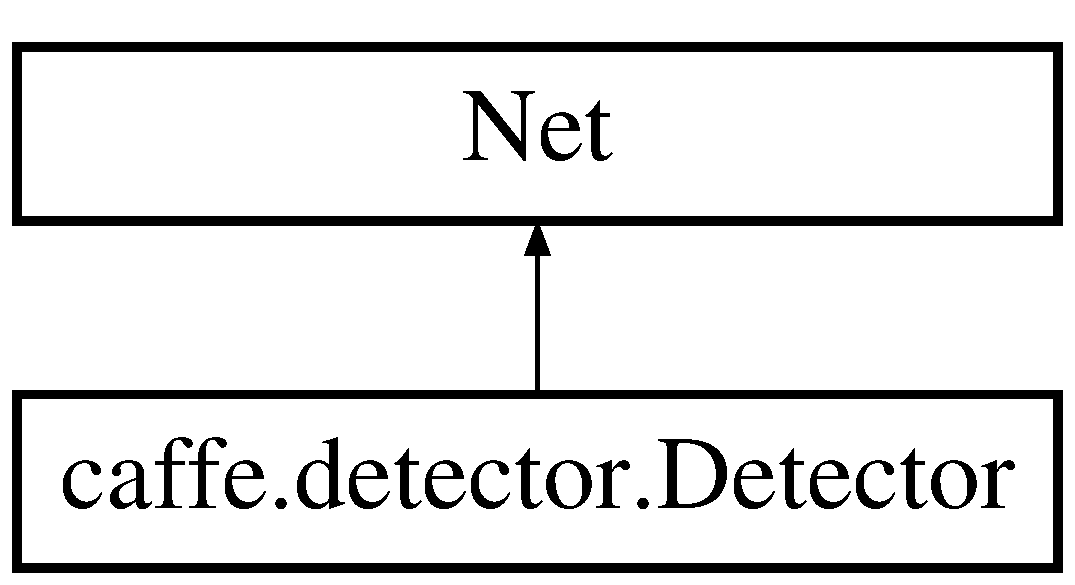
\includegraphics[height=2.000000cm]{classcaffe_1_1detector_1_1_detector}
\end{center}
\end{figure}
\subsection*{Public Member Functions}
\begin{DoxyCompactItemize}
\item 
\hypertarget{classcaffe_1_1detector_1_1_detector_a9b149cf7637926192c2033d61f34617d}{}def {\bfseries \+\_\+\+\_\+init\+\_\+\+\_\+}\label{classcaffe_1_1detector_1_1_detector_a9b149cf7637926192c2033d61f34617d}

\item 
def \hyperlink{classcaffe_1_1detector_1_1_detector_a7ddd403050bacd8fcccc62705f2405ff}{detect\+\_\+windows} (self, images\+\_\+windows)
\item 
def \hyperlink{classcaffe_1_1detector_1_1_detector_a2d96c53701abd37152c5f078a18ebf08}{detect\+\_\+selective\+\_\+search} (self, image\+\_\+fnames)
\item 
def \hyperlink{classcaffe_1_1detector_1_1_detector_af71bb7e173a228c2e1577b9125310216}{crop} (self, im, window)
\item 
def \hyperlink{classcaffe_1_1detector_1_1_detector_a3706bb8bcd04387c065f7bb6b34f4875}{configure\+\_\+crop} (self, context\+\_\+pad)
\end{DoxyCompactItemize}
\subsection*{Public Attributes}
\begin{DoxyCompactItemize}
\item 
\hypertarget{classcaffe_1_1detector_1_1_detector_a6ab029f8b9627cd96f11b935e263549f}{}{\bfseries transformer}\label{classcaffe_1_1detector_1_1_detector_a6ab029f8b9627cd96f11b935e263549f}

\item 
\hypertarget{classcaffe_1_1detector_1_1_detector_a6e914f9d5071a3d5a41f7542f216e6d9}{}{\bfseries crop\+\_\+dims}\label{classcaffe_1_1detector_1_1_detector_a6e914f9d5071a3d5a41f7542f216e6d9}

\item 
\hypertarget{classcaffe_1_1detector_1_1_detector_a25b10b7dedec3c75c589cfbffa1271af}{}{\bfseries context\+\_\+pad}\label{classcaffe_1_1detector_1_1_detector_a25b10b7dedec3c75c589cfbffa1271af}

\item 
\hypertarget{classcaffe_1_1detector_1_1_detector_a2caeb79b367cfca8577c4fddc53ac956}{}{\bfseries crop\+\_\+mean}\label{classcaffe_1_1detector_1_1_detector_a2caeb79b367cfca8577c4fddc53ac956}

\end{DoxyCompactItemize}


\subsection{Detailed Description}
\begin{DoxyVerb}Detector extends Net for windowed detection by a list of crops or
selective search proposals.

Parameters
----------
mean, input_scale, raw_scale, channel_swap : params for preprocessing
    options.
context_pad : amount of surrounding context to take s.t. a `context_pad`
    sized border of pixels in the network input image is context, as in
    R-CNN feature extraction.
\end{DoxyVerb}
 

\subsection{Member Function Documentation}
\hypertarget{classcaffe_1_1detector_1_1_detector_a3706bb8bcd04387c065f7bb6b34f4875}{}\index{caffe\+::detector\+::\+Detector@{caffe\+::detector\+::\+Detector}!configure\+\_\+crop@{configure\+\_\+crop}}
\index{configure\+\_\+crop@{configure\+\_\+crop}!caffe\+::detector\+::\+Detector@{caffe\+::detector\+::\+Detector}}
\subsubsection[{configure\+\_\+crop}]{\setlength{\rightskip}{0pt plus 5cm}def caffe.\+detector.\+Detector.\+configure\+\_\+crop (
\begin{DoxyParamCaption}
\item[{}]{self, }
\item[{}]{context\+\_\+pad}
\end{DoxyParamCaption}
)}\label{classcaffe_1_1detector_1_1_detector_a3706bb8bcd04387c065f7bb6b34f4875}
\begin{DoxyVerb}Configure crop dimensions and amount of context for cropping.
If context is included, make the special input mean for context padding.

Parameters
----------
context_pad : amount of context for cropping.
\end{DoxyVerb}
 \hypertarget{classcaffe_1_1detector_1_1_detector_af71bb7e173a228c2e1577b9125310216}{}\index{caffe\+::detector\+::\+Detector@{caffe\+::detector\+::\+Detector}!crop@{crop}}
\index{crop@{crop}!caffe\+::detector\+::\+Detector@{caffe\+::detector\+::\+Detector}}
\subsubsection[{crop}]{\setlength{\rightskip}{0pt plus 5cm}def caffe.\+detector.\+Detector.\+crop (
\begin{DoxyParamCaption}
\item[{}]{self, }
\item[{}]{im, }
\item[{}]{window}
\end{DoxyParamCaption}
)}\label{classcaffe_1_1detector_1_1_detector_af71bb7e173a228c2e1577b9125310216}
\begin{DoxyVerb}Crop a window from the image for detection. Include surrounding context
according to the `context_pad` configuration.

Parameters
----------
im: H x W x K image ndarray to crop.
window: bounding box coordinates as ymin, xmin, ymax, xmax.

Returns
-------
crop: cropped window.
\end{DoxyVerb}
 \hypertarget{classcaffe_1_1detector_1_1_detector_a2d96c53701abd37152c5f078a18ebf08}{}\index{caffe\+::detector\+::\+Detector@{caffe\+::detector\+::\+Detector}!detect\+\_\+selective\+\_\+search@{detect\+\_\+selective\+\_\+search}}
\index{detect\+\_\+selective\+\_\+search@{detect\+\_\+selective\+\_\+search}!caffe\+::detector\+::\+Detector@{caffe\+::detector\+::\+Detector}}
\subsubsection[{detect\+\_\+selective\+\_\+search}]{\setlength{\rightskip}{0pt plus 5cm}def caffe.\+detector.\+Detector.\+detect\+\_\+selective\+\_\+search (
\begin{DoxyParamCaption}
\item[{}]{self, }
\item[{}]{image\+\_\+fnames}
\end{DoxyParamCaption}
)}\label{classcaffe_1_1detector_1_1_detector_a2d96c53701abd37152c5f078a18ebf08}
\begin{DoxyVerb}Do windowed detection over Selective Search proposals by extracting
the crop and warping to the input dimensions of the net.

Parameters
----------
image_fnames: list

Returns
-------
detections: list of {filename: image filename, window: crop coordinates,
    predictions: prediction vector} dicts.
\end{DoxyVerb}
 \hypertarget{classcaffe_1_1detector_1_1_detector_a7ddd403050bacd8fcccc62705f2405ff}{}\index{caffe\+::detector\+::\+Detector@{caffe\+::detector\+::\+Detector}!detect\+\_\+windows@{detect\+\_\+windows}}
\index{detect\+\_\+windows@{detect\+\_\+windows}!caffe\+::detector\+::\+Detector@{caffe\+::detector\+::\+Detector}}
\subsubsection[{detect\+\_\+windows}]{\setlength{\rightskip}{0pt plus 5cm}def caffe.\+detector.\+Detector.\+detect\+\_\+windows (
\begin{DoxyParamCaption}
\item[{}]{self, }
\item[{}]{images\+\_\+windows}
\end{DoxyParamCaption}
)}\label{classcaffe_1_1detector_1_1_detector_a7ddd403050bacd8fcccc62705f2405ff}
\begin{DoxyVerb}Do windowed detection over given images and windows. Windows are
extracted then warped to the input dimensions of the net.

Parameters
----------
images_windows: (image filename, window list) iterable.
context_crop: size of context border to crop in pixels.

Returns
-------
detections: list of {filename: image filename, window: crop coordinates,
    predictions: prediction vector} dicts.
\end{DoxyVerb}
 

The documentation for this class was generated from the following file\+:\begin{DoxyCompactItemize}
\item 
caffe/detector.\+py\end{DoxyCompactItemize}

\hypertarget{structcaffe_1_1_ndarray_call_policies}{}\section{caffe\+:\+:Ndarray\+Call\+Policies Struct Reference}
\label{structcaffe_1_1_ndarray_call_policies}\index{caffe\+::\+Ndarray\+Call\+Policies@{caffe\+::\+Ndarray\+Call\+Policies}}
Inheritance diagram for caffe\+:\+:Ndarray\+Call\+Policies\+:\begin{figure}[H]
\begin{center}
\leavevmode
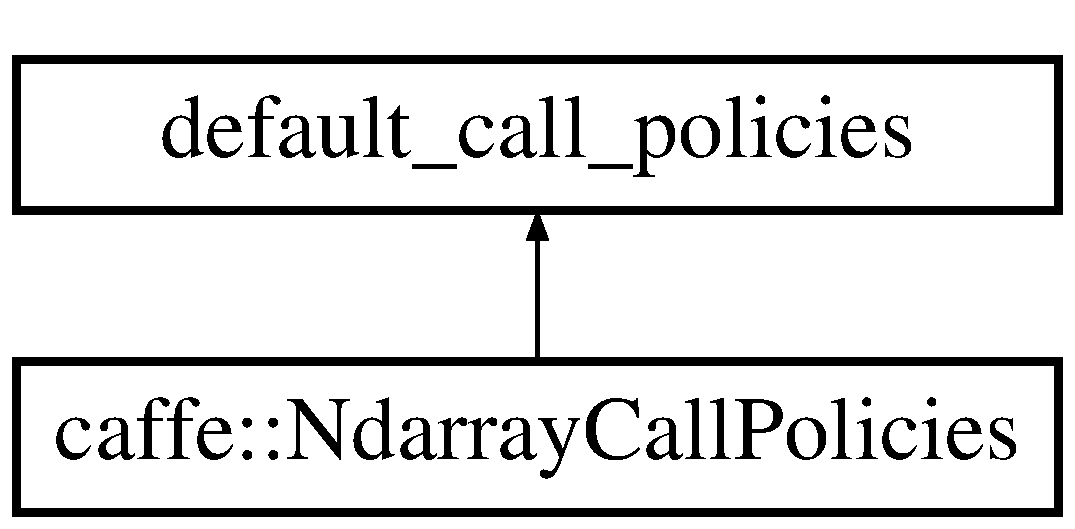
\includegraphics[height=2.000000cm]{structcaffe_1_1_ndarray_call_policies}
\end{center}
\end{figure}
\subsection*{Public Types}
\begin{DoxyCompactItemize}
\item 
\hypertarget{structcaffe_1_1_ndarray_call_policies_a810196d5439d3cede93f73998e1e2236}{}typedef \hyperlink{structcaffe_1_1_ndarray_converter_generator}{Ndarray\+Converter\+Generator} {\bfseries result\+\_\+converter}\label{structcaffe_1_1_ndarray_call_policies_a810196d5439d3cede93f73998e1e2236}

\end{DoxyCompactItemize}
\subsection*{Public Member Functions}
\begin{DoxyCompactItemize}
\item 
\hypertarget{structcaffe_1_1_ndarray_call_policies_ac1bb77e99e5a2f4bb556e582decf66da}{}Py\+Object $\ast$ {\bfseries postcall} (Py\+Object $\ast$pyargs, Py\+Object $\ast$result)\label{structcaffe_1_1_ndarray_call_policies_ac1bb77e99e5a2f4bb556e582decf66da}

\end{DoxyCompactItemize}


The documentation for this struct was generated from the following file\+:\begin{DoxyCompactItemize}
\item 
caffe/\+\_\+caffe.\+cpp\end{DoxyCompactItemize}

\hypertarget{structcaffe_1_1_ndarray_converter_generator}{}\section{caffe\+:\+:Ndarray\+Converter\+Generator Struct Reference}
\label{structcaffe_1_1_ndarray_converter_generator}\index{caffe\+::\+Ndarray\+Converter\+Generator@{caffe\+::\+Ndarray\+Converter\+Generator}}
\subsection*{Classes}
\begin{DoxyCompactItemize}
\item 
struct \hyperlink{structcaffe_1_1_ndarray_converter_generator_1_1apply}{apply}
\item 
struct \hyperlink{structcaffe_1_1_ndarray_converter_generator_1_1apply_3_01_dtype_01_5_01_4}{apply$<$ Dtype $\ast$ $>$}
\end{DoxyCompactItemize}


The documentation for this struct was generated from the following file\+:\begin{DoxyCompactItemize}
\item 
caffe/\+\_\+caffe.\+cpp\end{DoxyCompactItemize}

\hypertarget{classtest__python__layer_1_1_simple_layer}{}\section{test\+\_\+python\+\_\+layer.\+Simple\+Layer Class Reference}
\label{classtest__python__layer_1_1_simple_layer}\index{test\+\_\+python\+\_\+layer.\+Simple\+Layer@{test\+\_\+python\+\_\+layer.\+Simple\+Layer}}
Inheritance diagram for test\+\_\+python\+\_\+layer.\+Simple\+Layer\+:\begin{figure}[H]
\begin{center}
\leavevmode
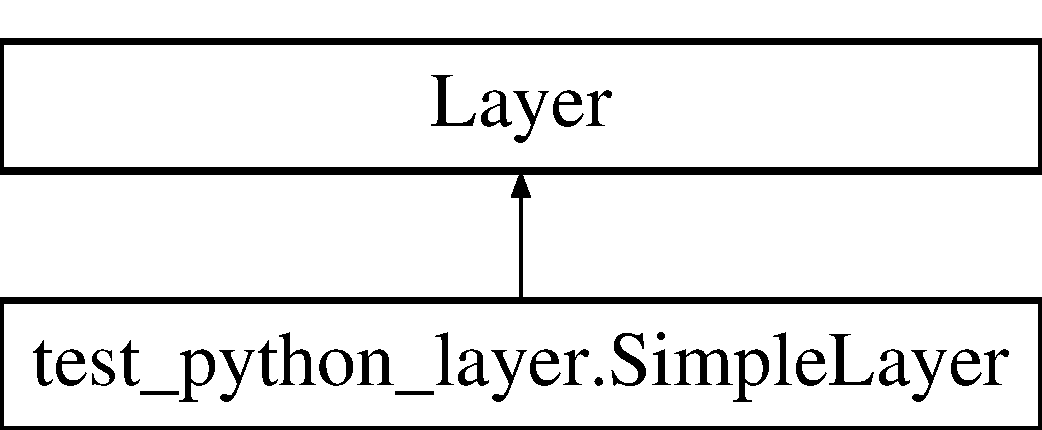
\includegraphics[height=2.000000cm]{classtest__python__layer_1_1_simple_layer}
\end{center}
\end{figure}
\subsection*{Public Member Functions}
\begin{DoxyCompactItemize}
\item 
\hypertarget{classtest__python__layer_1_1_simple_layer_a771c50bd471ec42b45321da08356e0c1}{}def {\bfseries setup} (self, bottom, top)\label{classtest__python__layer_1_1_simple_layer_a771c50bd471ec42b45321da08356e0c1}

\item 
\hypertarget{classtest__python__layer_1_1_simple_layer_a7e92ab7e8cee5f59db80f0e043578ab7}{}def {\bfseries reshape} (self, bottom, top)\label{classtest__python__layer_1_1_simple_layer_a7e92ab7e8cee5f59db80f0e043578ab7}

\item 
\hypertarget{classtest__python__layer_1_1_simple_layer_ac2ed0d5bf9321df89f8e5f952955b2a0}{}def {\bfseries forward} (self, bottom, top)\label{classtest__python__layer_1_1_simple_layer_ac2ed0d5bf9321df89f8e5f952955b2a0}

\item 
\hypertarget{classtest__python__layer_1_1_simple_layer_a89f9105c5080d5677bd59e935b99eac7}{}def {\bfseries backward} (self, top, propagate\+\_\+down, bottom)\label{classtest__python__layer_1_1_simple_layer_a89f9105c5080d5677bd59e935b99eac7}

\end{DoxyCompactItemize}


\subsection{Detailed Description}
\begin{DoxyVerb}A layer that just multiplies by ten\end{DoxyVerb}
 

The documentation for this class was generated from the following file\+:\begin{DoxyCompactItemize}
\item 
caffe/test/test\+\_\+python\+\_\+layer.\+py\end{DoxyCompactItemize}

\hypertarget{classtest__net_1_1_test_net}{}\section{test\+\_\+net.\+Test\+Net Class Reference}
\label{classtest__net_1_1_test_net}\index{test\+\_\+net.\+Test\+Net@{test\+\_\+net.\+Test\+Net}}
Inheritance diagram for test\+\_\+net.\+Test\+Net\+:\begin{figure}[H]
\begin{center}
\leavevmode
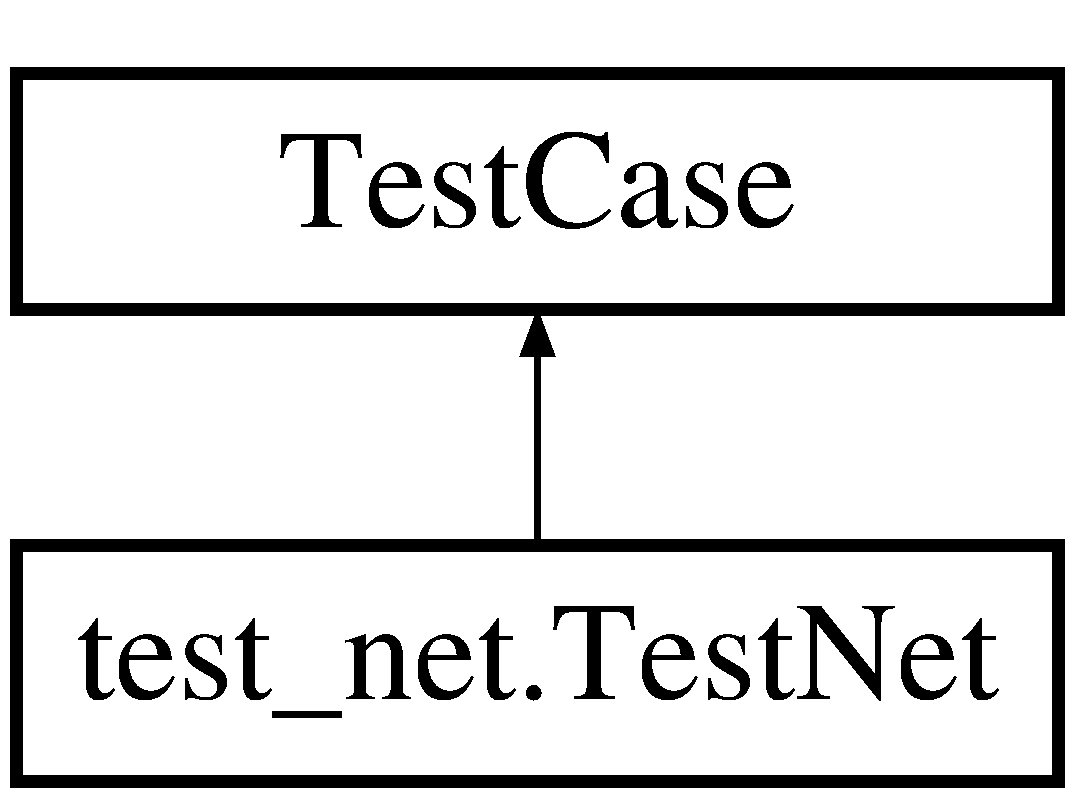
\includegraphics[height=2.000000cm]{classtest__net_1_1_test_net}
\end{center}
\end{figure}
\subsection*{Public Member Functions}
\begin{DoxyCompactItemize}
\item 
\hypertarget{classtest__net_1_1_test_net_a864f6fa941b5e7f59b9eee6a676f9604}{}def {\bfseries set\+Up} (self)\label{classtest__net_1_1_test_net_a864f6fa941b5e7f59b9eee6a676f9604}

\item 
def \hyperlink{classtest__net_1_1_test_net_a124e87079f074a8333dd71e9742e6118}{test\+\_\+memory} (self)
\item 
\hypertarget{classtest__net_1_1_test_net_a193ec22a0394c6df9e8c0143c7768462}{}def {\bfseries test\+\_\+forward\+\_\+backward} (self)\label{classtest__net_1_1_test_net_a193ec22a0394c6df9e8c0143c7768462}

\item 
\hypertarget{classtest__net_1_1_test_net_a98366efc38e1ebc3346b33c73159624b}{}def {\bfseries test\+\_\+inputs\+\_\+outputs} (self)\label{classtest__net_1_1_test_net_a98366efc38e1ebc3346b33c73159624b}

\item 
\hypertarget{classtest__net_1_1_test_net_aa7d8ffffb4ba5827744bb22a79135fe7}{}def {\bfseries test\+\_\+save\+\_\+and\+\_\+read} (self)\label{classtest__net_1_1_test_net_aa7d8ffffb4ba5827744bb22a79135fe7}

\end{DoxyCompactItemize}
\subsection*{Public Attributes}
\begin{DoxyCompactItemize}
\item 
\hypertarget{classtest__net_1_1_test_net_a99560ae34dd066167207d66a4a895a8e}{}{\bfseries num\+\_\+output}\label{classtest__net_1_1_test_net_a99560ae34dd066167207d66a4a895a8e}

\item 
\hypertarget{classtest__net_1_1_test_net_ac07e8487d9fb78ea828aa890f09c2bff}{}{\bfseries net}\label{classtest__net_1_1_test_net_ac07e8487d9fb78ea828aa890f09c2bff}

\end{DoxyCompactItemize}


\subsection{Member Function Documentation}
\hypertarget{classtest__net_1_1_test_net_a124e87079f074a8333dd71e9742e6118}{}\index{test\+\_\+net\+::\+Test\+Net@{test\+\_\+net\+::\+Test\+Net}!test\+\_\+memory@{test\+\_\+memory}}
\index{test\+\_\+memory@{test\+\_\+memory}!test\+\_\+net\+::\+Test\+Net@{test\+\_\+net\+::\+Test\+Net}}
\subsubsection[{test\+\_\+memory}]{\setlength{\rightskip}{0pt plus 5cm}def test\+\_\+net.\+Test\+Net.\+test\+\_\+memory (
\begin{DoxyParamCaption}
\item[{}]{self}
\end{DoxyParamCaption}
)}\label{classtest__net_1_1_test_net_a124e87079f074a8333dd71e9742e6118}
\begin{DoxyVerb}Check that holding onto blob data beyond the life of a Net is OK\end{DoxyVerb}
 

The documentation for this class was generated from the following file\+:\begin{DoxyCompactItemize}
\item 
caffe/test/test\+\_\+net.\+py\end{DoxyCompactItemize}

\hypertarget{classtest__python__layer_1_1_test_python_layer}{}\section{test\+\_\+python\+\_\+layer.\+Test\+Python\+Layer Class Reference}
\label{classtest__python__layer_1_1_test_python_layer}\index{test\+\_\+python\+\_\+layer.\+Test\+Python\+Layer@{test\+\_\+python\+\_\+layer.\+Test\+Python\+Layer}}
Inheritance diagram for test\+\_\+python\+\_\+layer.\+Test\+Python\+Layer\+:\begin{figure}[H]
\begin{center}
\leavevmode
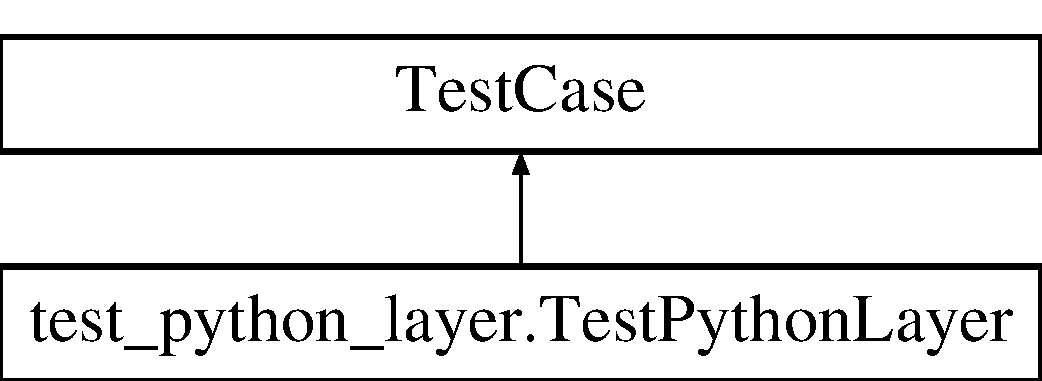
\includegraphics[height=2.000000cm]{classtest__python__layer_1_1_test_python_layer}
\end{center}
\end{figure}
\subsection*{Public Member Functions}
\begin{DoxyCompactItemize}
\item 
\hypertarget{classtest__python__layer_1_1_test_python_layer_a92caa30cfd251d89a3b749732e32311a}{}def {\bfseries set\+Up} (self)\label{classtest__python__layer_1_1_test_python_layer_a92caa30cfd251d89a3b749732e32311a}

\item 
\hypertarget{classtest__python__layer_1_1_test_python_layer_a62f12e77e948803bb7e8ca991a61a400}{}def {\bfseries test\+\_\+forward} (self)\label{classtest__python__layer_1_1_test_python_layer_a62f12e77e948803bb7e8ca991a61a400}

\item 
\hypertarget{classtest__python__layer_1_1_test_python_layer_a412a085a926adef9cc07061c0920803d}{}def {\bfseries test\+\_\+backward} (self)\label{classtest__python__layer_1_1_test_python_layer_a412a085a926adef9cc07061c0920803d}

\item 
\hypertarget{classtest__python__layer_1_1_test_python_layer_ac51f16c7dc35da4db4843d8f33738180}{}def {\bfseries test\+\_\+reshape} (self)\label{classtest__python__layer_1_1_test_python_layer_ac51f16c7dc35da4db4843d8f33738180}

\end{DoxyCompactItemize}
\subsection*{Public Attributes}
\begin{DoxyCompactItemize}
\item 
\hypertarget{classtest__python__layer_1_1_test_python_layer_a512551c8f5cda5a451a198b1d73a8295}{}{\bfseries net}\label{classtest__python__layer_1_1_test_python_layer_a512551c8f5cda5a451a198b1d73a8295}

\end{DoxyCompactItemize}


The documentation for this class was generated from the following file\+:\begin{DoxyCompactItemize}
\item 
caffe/test/test\+\_\+python\+\_\+layer.\+py\end{DoxyCompactItemize}

\hypertarget{classtest__solver_1_1_test_solver}{}\section{test\+\_\+solver.\+Test\+Solver Class Reference}
\label{classtest__solver_1_1_test_solver}\index{test\+\_\+solver.\+Test\+Solver@{test\+\_\+solver.\+Test\+Solver}}
Inheritance diagram for test\+\_\+solver.\+Test\+Solver\+:\begin{figure}[H]
\begin{center}
\leavevmode
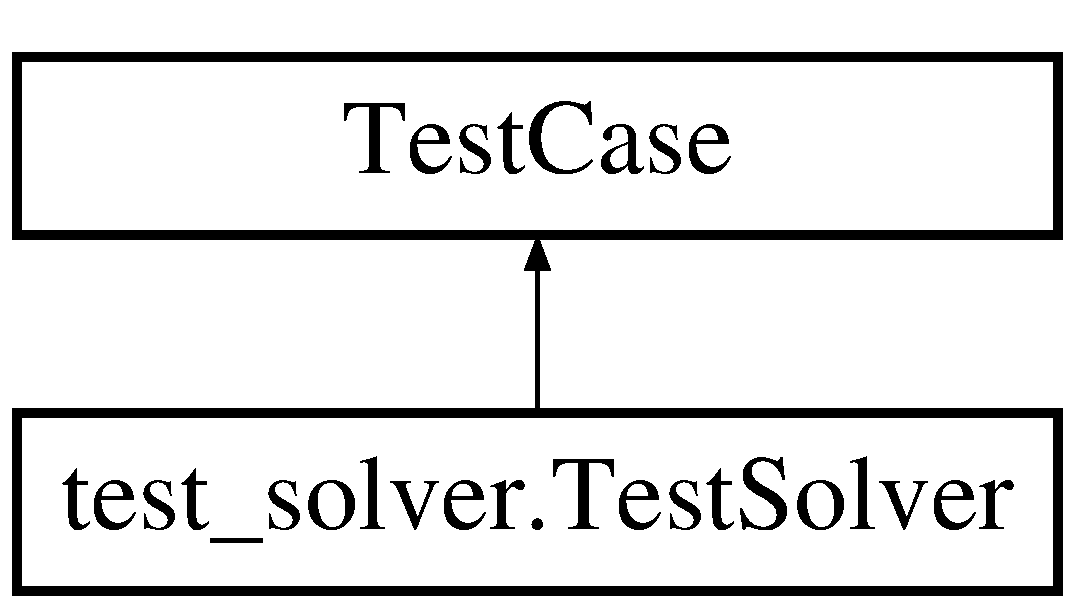
\includegraphics[height=2.000000cm]{classtest__solver_1_1_test_solver}
\end{center}
\end{figure}
\subsection*{Public Member Functions}
\begin{DoxyCompactItemize}
\item 
\hypertarget{classtest__solver_1_1_test_solver_ae66a20cbe4bee7698988c942f952d4a4}{}def {\bfseries set\+Up} (self)\label{classtest__solver_1_1_test_solver_ae66a20cbe4bee7698988c942f952d4a4}

\item 
\hypertarget{classtest__solver_1_1_test_solver_afee26d7e2697201c53619d45155cd201}{}def {\bfseries test\+\_\+solve} (self)\label{classtest__solver_1_1_test_solver_afee26d7e2697201c53619d45155cd201}

\item 
def \hyperlink{classtest__solver_1_1_test_solver_a96cd6dd0b2efecf67ee792f6f996a025}{test\+\_\+net\+\_\+memory} (self)
\end{DoxyCompactItemize}
\subsection*{Public Attributes}
\begin{DoxyCompactItemize}
\item 
\hypertarget{classtest__solver_1_1_test_solver_ae9727355daa663ba0a24cb7a28760b76}{}{\bfseries num\+\_\+output}\label{classtest__solver_1_1_test_solver_ae9727355daa663ba0a24cb7a28760b76}

\item 
\hypertarget{classtest__solver_1_1_test_solver_a85495400c6668028c584367ded1521e5}{}{\bfseries solver}\label{classtest__solver_1_1_test_solver_a85495400c6668028c584367ded1521e5}

\end{DoxyCompactItemize}


\subsection{Member Function Documentation}
\hypertarget{classtest__solver_1_1_test_solver_a96cd6dd0b2efecf67ee792f6f996a025}{}\index{test\+\_\+solver\+::\+Test\+Solver@{test\+\_\+solver\+::\+Test\+Solver}!test\+\_\+net\+\_\+memory@{test\+\_\+net\+\_\+memory}}
\index{test\+\_\+net\+\_\+memory@{test\+\_\+net\+\_\+memory}!test\+\_\+solver\+::\+Test\+Solver@{test\+\_\+solver\+::\+Test\+Solver}}
\subsubsection[{test\+\_\+net\+\_\+memory}]{\setlength{\rightskip}{0pt plus 5cm}def test\+\_\+solver.\+Test\+Solver.\+test\+\_\+net\+\_\+memory (
\begin{DoxyParamCaption}
\item[{}]{self}
\end{DoxyParamCaption}
)}\label{classtest__solver_1_1_test_solver_a96cd6dd0b2efecf67ee792f6f996a025}
\begin{DoxyVerb}Check that nets survive after the solver is destroyed.\end{DoxyVerb}
 

The documentation for this class was generated from the following file\+:\begin{DoxyCompactItemize}
\item 
caffe/test/test\+\_\+solver.\+py\end{DoxyCompactItemize}

\hypertarget{classcaffe_1_1io_1_1_transformer}{}\section{caffe.\+io.\+Transformer Class Reference}
\label{classcaffe_1_1io_1_1_transformer}\index{caffe.\+io.\+Transformer@{caffe.\+io.\+Transformer}}


Pre-\/processing.  


\subsection*{Public Member Functions}
\begin{DoxyCompactItemize}
\item 
\hypertarget{classcaffe_1_1io_1_1_transformer_aad3a0859254dddadbade7e60e624f855}{}def {\bfseries \+\_\+\+\_\+init\+\_\+\+\_\+} (self, inputs)\label{classcaffe_1_1io_1_1_transformer_aad3a0859254dddadbade7e60e624f855}

\item 
def \hyperlink{classcaffe_1_1io_1_1_transformer_a0b2d73743d661b36853fe3d963bd5fbb}{preprocess} (self, in\+\_\+, data)
\item 
def \hyperlink{classcaffe_1_1io_1_1_transformer_a3d048b7f8d255d29c04c2bcce0db318e}{deprocess} (self, in\+\_\+, data)
\item 
def \hyperlink{classcaffe_1_1io_1_1_transformer_af0acba3b0fe23e7fe33228600b18279a}{set\+\_\+transpose} (self, in\+\_\+, order)
\item 
def \hyperlink{classcaffe_1_1io_1_1_transformer_abd32a70aebb66e66de7567800547b114}{set\+\_\+channel\+\_\+swap} (self, in\+\_\+, order)
\item 
def \hyperlink{classcaffe_1_1io_1_1_transformer_aa02e06527de8f0e02d3065bf83b875a9}{set\+\_\+raw\+\_\+scale} (self, in\+\_\+, scale)
\item 
def \hyperlink{classcaffe_1_1io_1_1_transformer_a7064401b3aa295a6ab61895563a60d16}{set\+\_\+mean} (self, in\+\_\+, mean)
\item 
def \hyperlink{classcaffe_1_1io_1_1_transformer_ab3d72541298e2fb73a884df37e56f65c}{set\+\_\+input\+\_\+scale} (self, in\+\_\+, scale)
\end{DoxyCompactItemize}
\subsection*{Public Attributes}
\begin{DoxyCompactItemize}
\item 
\hypertarget{classcaffe_1_1io_1_1_transformer_a39504b59a20b17b063c896af4e0147a6}{}{\bfseries inputs}\label{classcaffe_1_1io_1_1_transformer_a39504b59a20b17b063c896af4e0147a6}

\item 
\hypertarget{classcaffe_1_1io_1_1_transformer_a0a2e0695edb3b47999ed4e9ae42771d4}{}{\bfseries transpose}\label{classcaffe_1_1io_1_1_transformer_a0a2e0695edb3b47999ed4e9ae42771d4}

\item 
\hypertarget{classcaffe_1_1io_1_1_transformer_aab33f13f4d564b0baddac568ff626e25}{}{\bfseries channel\+\_\+swap}\label{classcaffe_1_1io_1_1_transformer_aab33f13f4d564b0baddac568ff626e25}

\item 
\hypertarget{classcaffe_1_1io_1_1_transformer_a09f0e65ba030d5ded3dc5e3b229dd16f}{}{\bfseries raw\+\_\+scale}\label{classcaffe_1_1io_1_1_transformer_a09f0e65ba030d5ded3dc5e3b229dd16f}

\item 
\hypertarget{classcaffe_1_1io_1_1_transformer_a0a55c117f0577883e6d2c1251c01d16d}{}{\bfseries mean}\label{classcaffe_1_1io_1_1_transformer_a0a55c117f0577883e6d2c1251c01d16d}

\item 
\hypertarget{classcaffe_1_1io_1_1_transformer_a85c5851acbd0956a63742059b75df1c7}{}{\bfseries input\+\_\+scale}\label{classcaffe_1_1io_1_1_transformer_a85c5851acbd0956a63742059b75df1c7}

\end{DoxyCompactItemize}


\subsection{Detailed Description}
Pre-\/processing. 

\begin{DoxyVerb}Transform input for feeding into a Net.

Note: this is mostly for illustrative purposes and it is likely better
to define your own input preprocessing routine for your needs.

Parameters
----------
net : a Net for which the input should be prepared
\end{DoxyVerb}
 

\subsection{Member Function Documentation}
\hypertarget{classcaffe_1_1io_1_1_transformer_a3d048b7f8d255d29c04c2bcce0db318e}{}\index{caffe\+::io\+::\+Transformer@{caffe\+::io\+::\+Transformer}!deprocess@{deprocess}}
\index{deprocess@{deprocess}!caffe\+::io\+::\+Transformer@{caffe\+::io\+::\+Transformer}}
\subsubsection[{deprocess}]{\setlength{\rightskip}{0pt plus 5cm}def caffe.\+io.\+Transformer.\+deprocess (
\begin{DoxyParamCaption}
\item[{}]{self, }
\item[{}]{in\+\_\+, }
\item[{}]{data}
\end{DoxyParamCaption}
)}\label{classcaffe_1_1io_1_1_transformer_a3d048b7f8d255d29c04c2bcce0db318e}
\begin{DoxyVerb}Invert Caffe formatting; see preprocess().
\end{DoxyVerb}
 \hypertarget{classcaffe_1_1io_1_1_transformer_a0b2d73743d661b36853fe3d963bd5fbb}{}\index{caffe\+::io\+::\+Transformer@{caffe\+::io\+::\+Transformer}!preprocess@{preprocess}}
\index{preprocess@{preprocess}!caffe\+::io\+::\+Transformer@{caffe\+::io\+::\+Transformer}}
\subsubsection[{preprocess}]{\setlength{\rightskip}{0pt plus 5cm}def caffe.\+io.\+Transformer.\+preprocess (
\begin{DoxyParamCaption}
\item[{}]{self, }
\item[{}]{in\+\_\+, }
\item[{}]{data}
\end{DoxyParamCaption}
)}\label{classcaffe_1_1io_1_1_transformer_a0b2d73743d661b36853fe3d963bd5fbb}
\begin{DoxyVerb}Format input for Caffe:
- convert to single
- resize to input dimensions (preserving number of channels)
- transpose dimensions to K x H x W
- reorder channels (for instance color to BGR)
- scale raw input (e.g. from [0, 1] to [0, 255] for ImageNet models)
- subtract mean
- scale feature

Parameters
----------
in_ : name of input blob to preprocess for
data : (H' x W' x K) ndarray

Returns
-------
caffe_in : (K x H x W) ndarray for input to a Net
\end{DoxyVerb}
 \hypertarget{classcaffe_1_1io_1_1_transformer_abd32a70aebb66e66de7567800547b114}{}\index{caffe\+::io\+::\+Transformer@{caffe\+::io\+::\+Transformer}!set\+\_\+channel\+\_\+swap@{set\+\_\+channel\+\_\+swap}}
\index{set\+\_\+channel\+\_\+swap@{set\+\_\+channel\+\_\+swap}!caffe\+::io\+::\+Transformer@{caffe\+::io\+::\+Transformer}}
\subsubsection[{set\+\_\+channel\+\_\+swap}]{\setlength{\rightskip}{0pt plus 5cm}def caffe.\+io.\+Transformer.\+set\+\_\+channel\+\_\+swap (
\begin{DoxyParamCaption}
\item[{}]{self, }
\item[{}]{in\+\_\+, }
\item[{}]{order}
\end{DoxyParamCaption}
)}\label{classcaffe_1_1io_1_1_transformer_abd32a70aebb66e66de7567800547b114}
\begin{DoxyVerb}Set the input channel order for e.g. RGB to BGR conversion
as needed for the reference ImageNet model.
N.B. this assumes the channels are the first dimension AFTER transpose.

Parameters
----------
in_ : which input to assign this channel order
order : the order to take the channels.
    (2,1,0) maps RGB to BGR for example.
\end{DoxyVerb}
 \hypertarget{classcaffe_1_1io_1_1_transformer_ab3d72541298e2fb73a884df37e56f65c}{}\index{caffe\+::io\+::\+Transformer@{caffe\+::io\+::\+Transformer}!set\+\_\+input\+\_\+scale@{set\+\_\+input\+\_\+scale}}
\index{set\+\_\+input\+\_\+scale@{set\+\_\+input\+\_\+scale}!caffe\+::io\+::\+Transformer@{caffe\+::io\+::\+Transformer}}
\subsubsection[{set\+\_\+input\+\_\+scale}]{\setlength{\rightskip}{0pt plus 5cm}def caffe.\+io.\+Transformer.\+set\+\_\+input\+\_\+scale (
\begin{DoxyParamCaption}
\item[{}]{self, }
\item[{}]{in\+\_\+, }
\item[{}]{scale}
\end{DoxyParamCaption}
)}\label{classcaffe_1_1io_1_1_transformer_ab3d72541298e2fb73a884df37e56f65c}
\begin{DoxyVerb}Set the scale of preprocessed inputs s.t. the blob = blob * scale.
N.B. input_scale is done AFTER mean subtraction and other preprocessing
while raw_scale is done BEFORE.

Parameters
----------
in_ : which input to assign this scale factor
scale : scale coefficient
\end{DoxyVerb}
 \hypertarget{classcaffe_1_1io_1_1_transformer_a7064401b3aa295a6ab61895563a60d16}{}\index{caffe\+::io\+::\+Transformer@{caffe\+::io\+::\+Transformer}!set\+\_\+mean@{set\+\_\+mean}}
\index{set\+\_\+mean@{set\+\_\+mean}!caffe\+::io\+::\+Transformer@{caffe\+::io\+::\+Transformer}}
\subsubsection[{set\+\_\+mean}]{\setlength{\rightskip}{0pt plus 5cm}def caffe.\+io.\+Transformer.\+set\+\_\+mean (
\begin{DoxyParamCaption}
\item[{}]{self, }
\item[{}]{in\+\_\+, }
\item[{}]{mean}
\end{DoxyParamCaption}
)}\label{classcaffe_1_1io_1_1_transformer_a7064401b3aa295a6ab61895563a60d16}
\begin{DoxyVerb}Set the mean to subtract for centering the data.

Parameters
----------
in_ : which input to assign this mean.
mean : mean ndarray (input dimensional or broadcastable)
\end{DoxyVerb}
 \hypertarget{classcaffe_1_1io_1_1_transformer_aa02e06527de8f0e02d3065bf83b875a9}{}\index{caffe\+::io\+::\+Transformer@{caffe\+::io\+::\+Transformer}!set\+\_\+raw\+\_\+scale@{set\+\_\+raw\+\_\+scale}}
\index{set\+\_\+raw\+\_\+scale@{set\+\_\+raw\+\_\+scale}!caffe\+::io\+::\+Transformer@{caffe\+::io\+::\+Transformer}}
\subsubsection[{set\+\_\+raw\+\_\+scale}]{\setlength{\rightskip}{0pt plus 5cm}def caffe.\+io.\+Transformer.\+set\+\_\+raw\+\_\+scale (
\begin{DoxyParamCaption}
\item[{}]{self, }
\item[{}]{in\+\_\+, }
\item[{}]{scale}
\end{DoxyParamCaption}
)}\label{classcaffe_1_1io_1_1_transformer_aa02e06527de8f0e02d3065bf83b875a9}
\begin{DoxyVerb}Set the scale of raw features s.t. the input blob = input * scale.
While Python represents images in [0, 1], certain Caffe models
like CaffeNet and AlexNet represent images in [0, 255] so the raw_scale
of these models must be 255.

Parameters
----------
in_ : which input to assign this scale factor
scale : scale coefficient
\end{DoxyVerb}
 \hypertarget{classcaffe_1_1io_1_1_transformer_af0acba3b0fe23e7fe33228600b18279a}{}\index{caffe\+::io\+::\+Transformer@{caffe\+::io\+::\+Transformer}!set\+\_\+transpose@{set\+\_\+transpose}}
\index{set\+\_\+transpose@{set\+\_\+transpose}!caffe\+::io\+::\+Transformer@{caffe\+::io\+::\+Transformer}}
\subsubsection[{set\+\_\+transpose}]{\setlength{\rightskip}{0pt plus 5cm}def caffe.\+io.\+Transformer.\+set\+\_\+transpose (
\begin{DoxyParamCaption}
\item[{}]{self, }
\item[{}]{in\+\_\+, }
\item[{}]{order}
\end{DoxyParamCaption}
)}\label{classcaffe_1_1io_1_1_transformer_af0acba3b0fe23e7fe33228600b18279a}
\begin{DoxyVerb}Set the input channel order for e.g. RGB to BGR conversion
as needed for the reference ImageNet model.

Parameters
----------
in_ : which input to assign this channel order
order : the order to transpose the dimensions
\end{DoxyVerb}
 

The documentation for this class was generated from the following file\+:\begin{DoxyCompactItemize}
\item 
caffe/io.\+py\end{DoxyCompactItemize}

\hypertarget{structcaffe_1_1_ndarray_converter_generator_1_1apply_3_01_dtype_01_5_01_4_1_1type}{}\section{caffe\+:\+:Ndarray\+Converter\+Generator\+:\+:apply$<$ Dtype $\ast$ $>$\+:\+:type Struct Reference}
\label{structcaffe_1_1_ndarray_converter_generator_1_1apply_3_01_dtype_01_5_01_4_1_1type}\index{caffe\+::\+Ndarray\+Converter\+Generator\+::apply$<$ Dtype $\ast$ $>$\+::type@{caffe\+::\+Ndarray\+Converter\+Generator\+::apply$<$ Dtype $\ast$ $>$\+::type}}
\subsection*{Public Member Functions}
\begin{DoxyCompactItemize}
\item 
\hypertarget{structcaffe_1_1_ndarray_converter_generator_1_1apply_3_01_dtype_01_5_01_4_1_1type_a0be441e5e672c9039e91a58134d84c17}{}Py\+Object $\ast$ {\bfseries operator()} (Dtype $\ast$data) const \label{structcaffe_1_1_ndarray_converter_generator_1_1apply_3_01_dtype_01_5_01_4_1_1type_a0be441e5e672c9039e91a58134d84c17}

\item 
\hypertarget{structcaffe_1_1_ndarray_converter_generator_1_1apply_3_01_dtype_01_5_01_4_1_1type_a2458630718ae7c36deedeae759aacb92}{}const Py\+Type\+Object $\ast$ {\bfseries get\+\_\+pytype} ()\label{structcaffe_1_1_ndarray_converter_generator_1_1apply_3_01_dtype_01_5_01_4_1_1type_a2458630718ae7c36deedeae759aacb92}

\end{DoxyCompactItemize}


The documentation for this struct was generated from the following file\+:\begin{DoxyCompactItemize}
\item 
caffe/\+\_\+caffe.\+cpp\end{DoxyCompactItemize}

%--- End generated contents ---

% Index
\backmatter
\newpage
\phantomsection
\clearemptydoublepage
\addcontentsline{toc}{chapter}{Index}
\printindex

\end{document}
